\documentclass{article}
\usepackage[utf8]{inputenc}
\usepackage{amsmath}
\usepackage{amsfonts}
%\usepackage{bbold}
\usepackage{MnSymbol}
\usepackage{graphicx}
\usepackage{svg}
\usepackage{hyperref}
\usepackage{comment}
\usepackage{geometry}
\usepackage{subcaption}
\geometry{top=1in,bottom=1in,left=1in,right=1in}


\title{PHYS-467: Machine Learning for Physicists\\\Large Lecture Summary}
\author{Patrick Hirling}
\date{\today}

\begin{document}
\newgeometry{top=1in,bottom=1in,left=1in,right=1in}
\maketitle
\section{Bayesian Inference, Linear Models and Supervised Learning}
The philosophy of bayesian inference is to improve the a priori information one has about a parameter $\theta$ via observations or data.
Some basic concepts:
\begin{itemize}
    \item Conditional probability:
        \begin{equation}
            P(A|B) = \frac{P(A \cap B)}{P(B)}
        \end{equation}
    \item Bayes' Rule:
        \begin{equation}
            P(A|B) = \frac{P(B|A) P(A)}{P(B)}
        \end{equation}
\end{itemize}
In the case of inference, the typical problem is to estimate a set of parameters $\theta$ given some data $X$. Bayes' rule then reads
\begin{equation}
    P(\theta|X) = \frac{P(X|\theta) P(\theta)}{P(X)}.
\end{equation}
The elements of this formula are called
\begin{itemize}
    \item $P(\theta|X)$: The \emph{posterior distribution}: It encodes, in the Bayesian thinking, the best knowledge one has about $\theta$ given the observations $X$.
    \item $P(X|\theta)$: The \emph{likelihood}. This is often where one "chooses a model", by assuming that the data follows a certain probability distribution (gaussian, poissonian, exponential,...) of which $\theta$ are parameters.
    \item $P(\theta)$: The \emph{prior distribution}. This is the information one has about the parameters \emph{a priori}, that is, without any observations.
    \item $P(X)$: The \emph{evidence}. This is independent of $\theta$ and thus acts as a normalization constant for the posterior. 
\end{itemize}
The two most common \emph{estimators} for $\theta$ are:
\begin{enumerate}
    \item \textbf{Maximum Likelihood Estimator (MLE)}:
        \begin{equation*}
            \hat{\theta}_{\text{ML}}
            =
            \underset{\theta}{\text{argmax}} \left[ P(X|\theta) \right]
        \end{equation*}
    \item \textbf{Maximum A Posteriori Estimator (MAP)}:
        \begin{equation*}
            \hat{\theta}_{\text{MAP}}
            =
            \underset{\theta}{\text{argmax}} \left[ P(\theta|X) \right]
        \end{equation*}
\end{enumerate}
Formally, the MLE can be seen as a special case of MAP when the prior is a uniform distribution (i.e. $P(\theta) = const.$). In practice, one can in certain cases assume that with a lot of data, the posterior is dominated by the likelihood, making this a valid assumption.
\restoregeometry
\noindent In supervised learning, one is interested in situations where \dots Then, using the definition of conditional probability multiple times,
\begin{equation}
    P(\theta | X,y) = \frac{P(\theta,X,y)}{P(X,y)}
    =
    \frac{P(y|\theta,X)P(\theta,X)}{P(y|X)P(X)}
    =
    \frac{P(y|\theta,X)P(\theta|X)P(X)}{P(y|X)P(X)}
    =
    \frac{P(y|\theta,X)P(\theta|X)}{P(y|X)}.
    \label{eq:posterior}
\end{equation}
The elements of this formula inherit the names given above: $P(\theta | X,y)$ is the posterior, $P(y|\theta,X)$ the likelihood, $P(\theta|X)$ the prior and $P(y|X)$ the evidence. The estimators translate naturally to this context.
\subsection{Linear Models}
In the context of supervised machine learning, the following nomenclature will be used:
The \textbf{data} is represented by a matrix $X_{\mu i} \in \mathbb{R}^{n \times d}$ where $\mu = 1,\dots,n$ indexes the \textbf{sample} and $i = 1,\dots,d$ indexes the \textbf{feature}. To each data sample corresponds a \textbf{label} $y_{\mu} \in \mathbb{R}^n$. A \textbf{model} parametrized by a set of \textbf{weights} $w_i \in \mathbb{R}^d$ establishes a relationship between the data and the labels. Implicitely, one assumes that there is a set of \textbf{ground truth} weights $w_i^{\star}$ that represent the "true" values. The full \textbf{dataset} is in general split into a \textbf{training set}, which is used as the name suggests to train the model using the methods described in what follows, the \textbf{validation set}, used to fix so-called \textbf{hyperparameters} of the model, and a \textbf{test set}, used at the very end to evaluate the performance of the model on completely fresh data. The metrics used to evaluate performance are called \textbf{errors} or \textbf{losses} depending on the context and can take different forms depending on the system that is considered.

A \emph{generalized linear model} (GLM) assumes that the labels are generated from the data through some probability distribution parametrized by the ground truth weights:
\begin{equation}
    y_{\mu} \sim P_{out} (y_{\mu} | X_{\mu i} w^{\star}_i),
\end{equation}
where summation over repeated indices is implied from now on. Assuming that the weights are i.i.d. and independent of the data, one can then write for the posterior
\begin{equation}
    P(w | X,y)
    =
    \frac{P(y | w,X) P(w|X)}{P(y|X)}
    \sim
    \prod_{\mu = 1}^{n} P_{out} (y_{\mu} | X_{\mu i} w^{\star}_i)
    \prod_{j = 1}^{d} P(w_j),
    \label{eq:linearposterior}
\end{equation}
where terms independent of $w$ are treated as constants in the last step. One then defines the \emph{per-sample loss} and the \emph{regularization}:
\begin{align}
    l(y_{\mu}, X_{\mu i} w^{\star}_i)
    &\equiv
    - \ln \left[P_{out} (y_{\mu} | X_{\mu i} w^{\star}_i)\right]\\
    r(w_i) &\equiv
    - \ln \left[P(w_i) \right]
\end{align}
which together enter into the \emph{loss function}, defined as the negative logarithm of the posterior:

\begin{equation}
    \boxed{
        \mathcal{L}(w)
        \equiv
        - \ln \left[P(w | X,y)\right]
        =
        \frac{1}{n}\sum_{\mu = 1}^{n} l(y_{\mu}, X_{\mu i} w^{\star}_i)
        +
        \lambda \sum_{i=1}^{d} r(w_i).
    }
\end{equation}
Different conventions exist for the $1/n$ factor. The hyperparameter $\lambda$ parametrizes the strength of the regularization term. The two estimators defined previously then read
\begin{align}
    \hat{w}_{\text{MAP}} &= \underset{w}{\text{argmin }} \mathcal{L}(w) \\
    \hat{w}_{\text{ML}} &= \underset{w}{\text{argmin }} \frac{1}{n}\sum_{\mu = 1}^{n} l(y_{\mu}, X_{\mu i} w^{\star}_i),
\end{align}
i.e. the MLE is simply the MAP without regularization. The following are some of the most common concrete models.
\subsubsection*{Ridge Regression}
Ridge regression assumes that both the likelihood and the prior are gaussian,
\begin{align}
    P_{out} (y_{\mu} | X_{\mu i} w^{\star}_i)
    &=
    \frac{1}{\sqrt{2\pi}\Delta}e^{-\frac{1}{2\Delta^2} (y_{\mu} - X_{\mu} \cdot w)^2}
    \iff \left(y_{\mu} | X_{\mu i} w^{\star}_i\right) \sim \mathcal{N}(X_{\mu}\cdot w,\Delta^2) \\
    P(w_i) &=
    \frac{1}{\sqrt{2\pi}\sigma}e^{-\frac{1}{2\sigma^2}w_i^2}
    \iff w_i \sim \mathcal{N}(0,\sigma^2),
\end{align}
which leads to the one-sample loss
\begin{equation}
    l(y_{\mu}, X_{\mu i} w^{\star}_i)
    =
    (y_{\mu} - X_{\mu} \cdot w)^2,
\end{equation}
called the \emph{least-squares loss}. Similarly, for the regularization,
\begin{equation}
    r(w_i)
    =
    w_i^2,
\end{equation}
called \emph{$L_2$-regularization}. The full loss is
\begin{equation}
    \mathcal{L}_{\text{Ridge}}(w)
    =
    \frac{1}{n}\sum_{\mu = 1}^{n} (y_{\mu} - X_{\mu} \cdot w)^2
    +
    \lambda \sum_{i=1}^{d} w_i^2.
\end{equation}
\underline{Alternative Derivation}

\noindent Without the GLM framework, one typically arrives at the ridge or least squares regression model by the following argument: Assume that the labels $y$ can be described by a linear relationship between the data and a set of ground-truth weights and an additive gaussian noise,
\begin{equation}
    y_{\mu} = X_{\mu i} w_i^{\star} + \xi_{\mu},
    \quad \quad
    \xi_{\mu} \sim \mathcal{N}(0,\Delta^2).
\end{equation}
This means that $y_{\mu} \sim \mathcal{N}(y_{\mu}-X_{\mu i} w^{\star}_i,\Delta^2)$, and so the likelihood for a given set of weights $w$ and data $X$ is
\begin{equation}
    P(y|w,X)
    =
    \prod_{\mu=1}^{n}
    \frac{1}{\sqrt{2\pi}\Delta}e^{-\frac{1}{2\Delta^2} (y_{\mu} - X_{\mu} \cdot w)^2}
\end{equation}
If one further assumes that the ground-truth weights are also i.i.d normally distributed and are independent of the data, $w_i^{\star} \sim \mathcal{N}(0,\sigma^2)$, the prior is
\begin{equation}
    P(w|X)
    =
    \prod_{i=1}^{d}
    \frac{1}{\sqrt{2\pi}\sigma}e^{-\frac{1}{2\sigma^2}w_i^2}
\end{equation}
The posterior is then (Eq. \ref{eq:posterior}),
\begin{equation}
    P(w | X,y)
    =
    \frac{P(y | w,X) P(w|X)}{P(y|X)}
    \sim
    \prod_{\mu=1}^{n}
    \frac{1}{\sqrt{2\pi}\Delta}e^{-\frac{1}{2\Delta^2} (y_{\mu} - X_{\mu} \cdot w)^2}
    \prod_{i=1}^{d}
    \frac{1}{\sqrt{2\pi}\sigma}e^{-\frac{1}{2\sigma^2}w_i^2},
\end{equation}
which is the same as Eq. (\ref{eq:linearposterior}), and so the estimators yield the ordinary least-squares and $L_2$-regularized least squares estimators.
\subsubsection*{Robust Regression}
In this model, the Gaussian likelihood from before is replaced by a Laplacian one,
\begin{equation}
    P_{out} (y_{\mu} | X_{\mu i} w^{\star}_i)
    =
    \frac{\gamma}{2}e^{-\gamma |y_{\mu} - X_{\mu} \cdot w|},
\end{equation}
yielding the so-called \emph{Mean Absolute Error loss} (MAE):
\begin{equation}
    l(y_{\mu}, X_{\mu i} w^{\star}_i)
    =
    \gamma|y_{\mu} - X_{\mu} \cdot w|.
\end{equation}
A model using such a loss function is called robust because it is less sensitive to outliers in the data, as it is not quadratic.
\subsubsection*{Sparse Regression}
This time, the gaussian prior is replaced by a laplacian one,
\begin{equation}
    P(w_i)
    =
    \frac{\lambda}{2}e^{-\lambda |w_i|},
\end{equation}
which yields the LASSO-regularization,
\begin{equation}
    r(w_i) = |w_i|.
\end{equation}
The name comes from the fact that the full loss of least-squares with this regularization,
\begin{equation}
    \mathcal{L}_{\text{LASSO}}(w)
    \equiv
    \frac{1}{n}\sum_{\mu = 1}^{n} (y_{\mu} - X_{\mu} \cdot w)^2
    +
    \lambda \sum_{i=1}^{d} |w_i|,
\end{equation}
is called the \emph{Least Absolute Shrinkage and Selection Operator}. See figure 8 of the lecture notes for a visual intuition of what this regularization does. The main idea is that such a regularization induces sparsity in the weights, meaning that it tends to yield a set of weights $w$ where many $w_i=0$ and only a "few" are nonzero. In an inference context, this means that one can find out which features are the most "important" (variable selection). In a signal processing context (where $y$ is the measured signal, $X$ the source signal and $\xi$ the noise), it can be seen as a form of compression.

\subsection{Gradient Descent}
All the models introduced above boil down the problem of inference to the same task: minimizing a certain loss function $\mathcal{L}$. In the case of ridge regression, an analytical minimum exists and is given by
\begin{align}
    \hat{w}_{R} &=(X^TX)^{-1}X^Ty \quad\quad\text{(MLE)} \\
    \hat{w}_{R} &=(X^TX + \frac{\Delta^2}{\sigma^2}\mathbf{1})^{-1}X^Ty \quad\quad\text{(MAP)}.
\end{align}
Note that in the first case it is assumed that the \emph{covariance matrix} $X^TX$ is invertible, which is typically the case when $d\ll n$.
However, for more general loss functions, such as the ones that arise in nonlinear models like neural networks, another minimization technique is required. This is provided by the \emph{Gradient Descent} (GD) method. It is an universal iterative method that is initialized at some $w^0$ and then performs steps in the direction of the inverse gradient at that point, weighted by a hyperparameter called the \emph{learning rate} $\gamma$:
\begin{equation}
    w_i^{t+1} = w_i^{t} - \gamma\frac{\partial\mathcal{L}(w)}{\partial w_i}\bigg |_{w=w^t}.
\end{equation}
Formally, this means taylor-expanding the loss to second order, setting $\partial\mathcal{L}/\partial w = 0$. and approximating the second derivative by the constant $1/\gamma$. Visually, it means taking steps in the direction of the minimum of a parabola tangent to $\mathcal{L}$ at $w^t$ scaled by $\gamma$. It turns out that this method, although seemingly very approximate, is very effective when choosing a good learning rate.

Standard gradient descent has the disadvantages of 1. being computationally very expensive on large datasets, as the derivative of the loss involves a sum over all samples and 2. that it easily gets stuck in local minima of the loss. To mitigate these issues, variants of GD exist and are more commonly used in practice.
\subsubsection*{Stochastic Gradient Descent}
Rather than computing the gradient of the loss function over the whole dataset,
\begin{equation}
    \frac{\partial\mathcal{L}(w)}{\partial w_i}
    =
    \frac{1}{n}\sum_{\mu = 1}^{n} \frac{\partial l(y_{\mu}, X_{\mu i} w^{\star}_i)}{\partial w_i}
    +
    \lambda \sum_{i=1}^{d} \frac{\partial r(w_i)}{\partial w_i},
\end{equation}
which involves summing over all samples $\mu$ ($n$ is typically on the order $>10^3$), \emph{Stochastic Gradient Descent} (SGD) approximates the gradient by considering, at every iteration, only a random subset $B_t$ (a "batch") of the samples. Concretely,
\begin{equation}
    \frac{\partial\mathcal{L}(w)}{\partial w_i}
    \approx
    \frac{1}{|B_t|}\sum_{\mu \in B_t}^{n} \frac{\partial l(y_{\mu}, X_{\mu i} w^{\star}_i)}{\partial w_i}
    +
    \lambda \sum_{i=1}^{d} \frac{\partial r(w_i)}{\partial w_i}.
\end{equation}

\subsubsection*{Subgradient Descent}
This variant is typically used when using LASSO-regularizations, since their derivative yields a sign function of the weights that is undefined when they are 0. It works like GD but chooses a random value for $\partial r/\partial w_i$ when it doesn't exist.
\subsubsection*{Momentum Methods}
The idea here is to introduce "momentum" to the process, in the sense of keeping a memory of the previous iteration $w^{t-1}$ and take it into account when computing $w^{t+1}$. A common example of this is \emph{Adaptive Moment Estimation} (ADAM). See \href{https://en.wikipedia.org/wiki/Stochastic_gradient_descent#Momentum}{this link} for a more in-depth description.
\subsection{Features and the Bias-Variance Tradeoff}
So far a given data sample $X_{\mu}\in\mathbb{R}^d$ has simply been described as having $d$ features. These features may be concrete things like age, height, weight, etc., but could in principle also be functions of those values, as will be discussed later in the context of kernel methods and neural networks. In the context of the methods described above, a simple extension is \emph{polynomial regression}, where one adds features by considering powers of a "ground feature" $x$. The data matrix is then
\begin{equation}
    X =
    \begin{pmatrix}
        x_1^p & x_1^{p-1} & \dots & 1 \\
        x_2^p & x_2^{p-1} & \dots & 1 \\
        \vdots & \vdots & \ddots & \\
        x_{\mu}^p & x_{\mu}^{p-1} & \dots & 1
    \end{pmatrix}
    \in \mathbb{R}^{n\times (p+1)}.
\end{equation}
As a simple example, this can be used to fit a polynomial function of degree $p$ to some data. As the degree $p$ increases, the model may fit the data more and more closely, but at some point $p$ becomes too high and the model starts to fit the noise rather than the actual behaviour of interest. At this point, the generalizability of the model decreases, i.e. it less accurately extrapolates to new data. When plotting the performance (an error of some kind, like the RMSE) of the model on the train and test data, the training error will get lower and lower but the test error reaches a minimum and then increases again. This relationship between model complexity and generalizability is called the \emph{bias-variance tradeoff} and arises in all machine learning contexts. As will be seen with neural networks, there is a caveat to this conclusion (the double-descent phenomenon). One defines the terms as (copied from Wikipedia):
\begin{itemize}
    \item \textbf{Bias}: The bias error is an error from erroneous assumptions in the learning algorithm. High bias can cause an algorithm to miss the relevant relations between features and target outputs (underfitting).
    \item \textbf{Variance}: The variance is an error from sensitivity to small fluctuations in the training set. High variance may result from an algorithm modeling the random noise in the training data (overfitting).
\end{itemize}
\subsection{Linear Classification}
\subsubsection*{Two Classes}
The simplest case of linear classification 2-class classification. A set of points in a $p$-dimensional space are said to be \emph{linearly separable} if there exists at least one hyperplane $\pi \in \mathbb{R}^{p-1}$ that separates the points into two disjunct sets. The hyperplane may be parametrized by a vector $w^{\star} = (w_1^{\star} , w_2^{\star} , \dots , w_p^{\star}, b) \in \mathbb{R}^{p+1}$ and
\begin{equation}
    z = (z_1 , z_2 , \dots , z_p)
    \in \pi \iff \tilde{X}_i w_i = 0, \text{ where }
    \tilde{X} = (z,1).
\end{equation}
Considering now a set of $n$ datapoints $X_{\mu i} \in \mathbb{R}^{n \times d}$,
\begin{equation}
    X =
    \begin{pmatrix}
        x_{1 1} & x_{1 2} & \dots & x_{1 p} & 1 \\
        x_{2 1} & x_{2 2} & \dots & x_{2 p} & 1 \\
        \vdots & \vdots & \ddots & \\
        x_{\mu 1} & x_{\mu 2} & \dots & x_{\mu p} & 1
    \end{pmatrix}
    \in \mathbb{R}^{n\times d} \quad \quad (d=p+1),
\end{equation}
one can consider labels $y_{\mu}\in \mathbb{R}^{d}$ that are $\pm 1$ depending on the side of the hyperplane the corresponding data point is:
\begin{align*}
    X_{\mu i} w_i > 0 \iff y_{\mu} &= +1 \\
    X_{\mu i} w_i < 0 \iff y_{\mu} &= -1,
\end{align*}
or simply $y_{\mu} = \text{sign}(X_{\mu i} w_i)$. The problem of linear classification then reduces to a regression problem of minimizing some loss $\mathcal{L}(w)$. One first needs to define a probabilistic model. A common one\footnote{See \url{https://en.wikipedia.org/wiki/Logistic_regression\#Definition} for more details} is
\begin{equation}
    P_{out} (y_{\mu} | X_{\mu i} w^{\star}_i)
    =
    \frac{e^{y_{\mu} X_{\mu i} w^{\star}_i}}{e^{X_{\mu i} w^{\star}_i} + e^{-X_{\mu i} w^{\star}_i}}
    \quad\quad \text{(No summation over $\mu$)},
    \label{eq:logisticlikelihood}
\end{equation}
which yields the one-sample loss
\begin{equation}
    l_{logit}(y_{\mu}, X_{\mu i} w^{\star}_i)
    =
    \ln\left(1+e^{-y_{\mu} X_{\mu i} w^{\star}_i}\right)
    \quad\quad \text{(No summation over $\mu$)},
\end{equation}
called the \emph{logistic loss}. Its associated MLE is
\begin{equation}
    \hat{w}_{\text{ML}} = \underset{w}{\text{argmin }} \frac{1}{n}\sum_{\mu = 1}^{n}
    \ln\left(1+e^{-y_{\mu} X_{\mu i} w^{\star}_i}\right).
\end{equation}
One can (and should) also add a regularization term, as before. Other losses exist, which come from other likelihoods. A common example is the \emph{hinge loss}:
\begin{equation}
    l_{hinge}(y_{\mu}, X_{\mu i} w^{\star}_i)
    =
    \max (0,1-y_{\mu} X_{\mu i} w^{\star}_i)
    \quad\quad \text{(No summation over $\mu$)}.
\end{equation}
\subsubsection*{$K$-Classes}
One can imagine comparing "one class vs the rest" and reduce the situation to a two-class problem, which is typically done with e.g. the hinge loss. However, the logistic loss framework of above can be extended. The data is \emph{one-hot encoded}: For a sample $X_{\mu}$ belonging to the $b$-th class, one defines the label as
\begin{equation}
    y_{\mu a} = 1 \text{ if } a=b,\quad y_{\mu a} = 0 \text{ if } a\neq b.
\end{equation}
One then has $y_{\mu a} \in \mathbb{R}^{n\times K}$ and defines, correspondingly, the weights $w_{i a} \in \mathbb{R}^{d\times K}$. Let $$p_{\mu a} = P(y_{\mu a} = 1| X_{\mu i} w^{\star}_{ia})$$ be the probability that sample $\mu$ is in the category $a$, given the data and the weights (to be defined below). The following model for the whole label then seems reasonable:
\begin{equation}
    P_{out}(y_{\mu}| X_{\mu i} w^{\star}_i)
    =
    \prod_{a=1}^{K} \mathbf{1}(y_{\mu a}=1) p_{\mu a}
    =
    \prod_{a=1}^{K} p_{\mu a}^{y_{\mu a}}.
\end{equation}
This model leads to the so-called \emph{cross-entropy loss}:
\begin{equation}
    \mathcal{L}_{CE}(w)
    =
    -\frac{1}{n} \sum_{\mu = 1}^{n}\sum_{a=1}^{K}
    y_{\mu a} \ln{p_{\mu a}}.
\end{equation}
In analogy with Eq. (\ref{eq:logisticlikelihood}), the $p_{\mu a}$ are given by
\begin{equation}
    p_{\mu a}
    =
    \frac{e^{X_{\mu i} w^{\star}_{ia}}}{\sum_{b=1}^{K} e^{X_{\mu i} w^{\star}_{ib}}}
    \equiv
    \text{softmax}(X_{\mu i} w^{\star}_{ia}).
    \label{eq:softmax}
\end{equation}
This model, classification of samples into $K$ classes where the belonging probabilities are given by the softmax function, is called \emph{multinomial logistic regression}. The simple 2-class logistic regression can be seen as a special case with the substitutions $-1\rightarrow 0$ and $+1\rightarrow 1$.

\newpage
\section{Dimensionality Reduction, Monte-Carlo Methods and Unsupervised Learning}
Rather than learning from data with labels and being able to predict outcomes on new data (supervised learning), \emph{unsupervised learning} methods aim to discover "on their own" patterns in unlabeled data. Examples include finding clusters in data, low-rank matrix completion in recommendation systems, etc. A common task of unsupervised learning is \emph{dimensionality reduction}, that is, given a high dimensional dataset $X_{\mu} \in \mathbb{R}^d$, find a representation of this data in a lower-dimensional space $\mathbb{R}^k$ with $k\ll d$.

\subsection{Principal Component Analysis (PCA)}
The idea of PCA is to perform an orthogonal change of coordinates on the data such that in the new coordinate system it has the most variance in the first dimension, the second-most variance in the second dimension, and so on, as illustrated for a 2D case in Fig. (\ref{fig:pca}). The method by which this is achieved is most conveniently defined in terms of another method, \emph{Singular Value Decomposition} (SVD).
\begin{figure}[h]
    \centering
    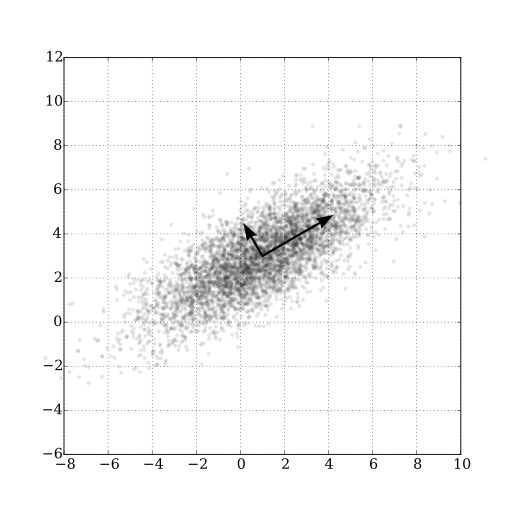
\includegraphics[width=0.5\linewidth]{PCA}
    \caption{Illustration of PCA on a multivariate gaussian scatter in 2D (By Nicoguaro - Own work, CC BY 4.0, \url{https://commons.wikimedia.org/w/index.php?curid=46871195}). The black arrows represent the coordinate system constructed from the 2 right singular vectors of the data, and their length represents the size of their associated singular value.}
    \label{fig:pca}
\end{figure}
\subsubsection*{Singular Value Decomposition}
Let $X \in \mathbb{R}^{n\times d}$ be a non-symmetric data matrix. The SVD of $X$ is obtained by writing it as
\begin{equation}
    X = U\Sigma V^T,
    \label{eq:svd}
\end{equation}
where $U\in \mathbb{R}^{n\times n}$ and $V\in \mathbb{R}^{d\times d}$ are real orthonormal matrices and $\Sigma \in \mathbb{R}^{n\times d}$ is a rectangular diagonal matrix with non-negative real elements $\Sigma_{ii} = \sigma_i \geq 0$, called \emph{singular values} of $X$. The columns of $U$ are called \emph{left singular vectors} and the rows of $V^T$ \emph{right singular vectors}. The following holds:
\begin{equation}
    \text{rank}(X) = \sum_{i} \mathbf{1}(\sigma_i > 0)
    \leq \min(n,d).
\end{equation}
Also, from \ref{eq:svd}, the \emph{covariance matrix} $X^TX$ can be written as
\begin{align}
    X^TX &=
    V\Sigma^T U^T U\Sigma V^T
    =
    V\Lambda V^T
\end{align}
where $\Lambda = \Sigma^T\Sigma$ is a square $d\times d$ diagonal matrix with entries $\sigma_i^2$,
\begin{equation}
    \Sigma =
    \begin{pmatrix}
        \sigma_1 & 0 & \ldots & 0 \\
        0 & \sigma_2 &  & \vdots \\
        \vdots & & \ddots & 0 \\
        0 &  \dots & \dots&   \sigma_d \\
        0 &  \dots & \dots&   0 \\
        \vdots & & &   \vdots \\
        0 &  \dots & \dots &   0
    \end{pmatrix}
    \quad \implies \quad
    \Sigma^T\Sigma =
    \begin{pmatrix}
        \sigma_1^2 &  & 0 \\
        & \ddots & \\
        0 & &\sigma_d^2
    \end{pmatrix}
    \equiv \Lambda.
\end{equation}
Hence, the eigenvectors of the covariance matrix are the right-singular vectors of $X$, while the square root of its eigenvalues are the singular values of $X$. The \textbf{Young-Eckhart-Mirsky Theorem} states that the best \emph{rank-$k$ approximation} $X^{(k)}$ of $X$ in the sense of minimizing the Frobenius norm of their difference
$ || X^{(k)} - X ||_F$ is given by
\begin{equation}
    X_{\mu i}^{(k)}
    =
    \sum_{s=1}^{k} U_{\mu s} \sigma_s V_{i s},
\end{equation}
where the sum goes over the $k$ largest singular values $\sigma_s$. 

\subsubsection*{PCA and Dimensionality Reduction}
The principal component decomposition of order $k\leq d$ of $X$ is the new matrix $T^{(k)} \in \mathbb{R}^{n\times k}$ defined by
\begin{equation}
    T^{(k)} = XV^{(k)},
\end{equation}
where $V^{(k)} \in \mathbb{R}^{d\times k}$ is a matrix whose columns are the $k$ right-singular vectors of $X$ corresponding to the $k$ largest singular values. $T^{(k)}$ represents a new version of the data whose dimensionality has been reduced to $k$ from $d$, in a way that ensures that as much information as possible has been retained in the process, as guaranteed by the YEM theorem. In a more informal way, what PCA does is
\begin{enumerate}
    \item Compute the SVD of $X$ and find its singular values and right-singular vectors.
    \item Order the right singular vectors by their associated singular value, from highest to lowest.
    \item Project the data $X$ on the coordinate system formed by the $k$ first of these vectors to form $T$, the transformed $k$-dimensional data.
\end{enumerate}
Since the PCA is an orthogonal transformation, the projection is geometrically just a rotation. Moreover, in general, the data are first centered and normalized so that their mean is 0 and their variance 1. Determining how many principal components to keep (i.e. the value of $k$) depends on the problem at hand, but a basic strategy is to plot a histogram of the eigenvalues of $X^TX$ and look at its structure: if there are a few eigenvalues visibly larger than the bulk, this number is in general a good guess for $k$.
%where $U_{\mu s}$ is the $s$-th left-singular vector, $V_{i s}$ the $s$-th right-singular vector and $\sigma_s$ the $s$-th singular value of $X$.

\subsection{Bayesian Estimation}
Previously, the two most common estimators - the ML and MAP - have been introduced. Both of these estimators are \emph{pointwise}, that is, they provide a single value given by the maximum of some probability distribution, which is in general found numerically. Here, a more general framework with a wide range of applications is introduced.

Let $X$ be some data, $\theta$ a parameter we wish to estimate, $\hat{\theta}(X)$ an estimator of this parameter and $L(\theta,\hat{\theta})$ a loss function. A \emph{Bayes estimator} is an estimator that minimizes the \emph{posterior expected loss}, that is,
\begin{equation}
    \hat{\theta}_{\text{Bayes}} = \underset{\hat{\theta}}{\text{argmin}}\left[
    E(L(\theta,\hat{\theta}) | X)\right],
\end{equation}
noting that $E$ represents a conditional expectation over $\theta$ given $X$.
More informally, one does Bayes estimation when one has access to the whole posterior, in the sense of being able to compute statistical moments (mean, variance,covariance,etc.) on it.
\begin{itemize}
    \item In the basic ML/MAP estimators, we define a loss function from the posterior and numerically find its minimum via GD or its variants.
    \item In Bayes estimation, we get a view of the whole landscape of the posterior (which may include multiple maxima) and based on that, compute quantities, typically the mean and variance of the parameters. This gives a more complete picture of the information we have about the parameters.
\end{itemize}

\subsubsection*{Minimum Mean Square Error}
The most common example for the above is by taking the mean square error (MSE) as the loss function. Then, the Bayes estimator is
\begin{equation}
    \hat{\theta}_{\text{MMSE}} =
    \underset{\hat{\theta}}{\text{argmin }} E\left[(\hat{\theta} - \theta)^2 | X \right],
\end{equation}
where the expectation is taken over the posterior $(\theta | X)$ and \textbf{not} the prior:
\begin{equation}
    E\left[(\hat{\theta} - \theta)^2  | X\right]
    =
    \int P(\theta | X) (\hat{\theta} - \theta)^2 d\theta.
\end{equation}
The minimum of this expression can be found by takng a formal derivative:
\begin{align}
    \frac{\partial}{\partial \hat{\theta}}
    E\left[(\hat{\theta} - \theta)^2 \right]
    = 2\int P(\theta | X) (\hat{\theta} - \theta) d\theta
    &\overset{!}{=} 0 \\
    \implies
    \int  P(\theta | X) \hat{\theta} d\theta
    - \int  P(\theta | X) \theta d\theta &= 0 \\
    \implies
    \hat{\theta} = \int P(\theta | X)\theta d\theta
    &\equiv E\left[ \theta | X\right],
\end{align}
since the prior is normalized to 1. Hence, \textbf{the MMSE is just the mean of the posterior}! The discrete form of the above is
\begin{equation}
    \hat{\theta} = E\left[ \theta | X\right]
    =
    \sum_{\theta} P(\theta | X)\theta.
\end{equation}
When, instead of a scalar parameter $\theta$ one has a set of parameters or latent variables\footnote{A \emph{latent variable} is similar to a parameter in that it is a variable that cannot be observed but only infered from the data. An example is the vector $S$ in the spin glass card game used in the lecture. While $S$ is used as notation in Eq. (\ref{eq:mmse_theta}) and the following, the same ideas apply if one has a vector of parameters and not latent variables.} $S \in \mathbb{R}^N$, the above becomes
\begin{equation}
    \hat{S_j}
    =
    %\sum_{\{S_i\}_{i=1}^N} P(S | X)S_j,
    \sum_{S \in \mathcal{S}} P(S | X)S_j,
    \label{eq:mmse_theta}
\end{equation}
and the sum now runs over the space $\mathcal{S}$ of all \emph{configurations} of $S$, and $S_j$ in the sum is the $j$-th entry of $S$ in the current configuration. If we have an analytic expression for the posterior $P(S|X)$, one could imagine computing Eq. (\ref{eq:mmse_theta}) directly by computing it for every $S\in\mathcal{S}$, but this is generally unfeasible. In the example of the spin glass game discussed in the lecture, $S$ is a vector of length $N$ where each entry can take 2 values. Summing over all its configurations would amount to considering $2^N$ configurations, which is unfeasible already if $N=100$.
%This means that another approach is required for calculating these sums/integrals.

The above is only one example of a situation where one needs to compute some statistical quantity from a known distribution, but can neither find an analytical expression for said quantity nor calculate it explicitely due to the large number of terms to consider. An alternative method for dealing with this type of computations is required, and is provided by \emph{Monte-Carlo} methods.

\subsection{Monte-Carlo Methods}
The main idea of MC methods is to use random sampling to approximate an analytical expression. In the case at hand, the expression we wish to compute is a sum of values weighted by a probability. If we had a way of drawing samples of $S$ that follow its posterior distribution, we could then imagine approximating the sum by summing a large enough number $T$ of samples. This would put more weight on the configurations of $S$ for which the posterior is larger, just like in the original sum in Eq. (\ref{eq:mmse_theta}):
\begin{equation}
    \hat{S_j}
    \approx
    \frac{1}{T}
    \sum_{t=1}^{N} S_j^{(t)}
    =
    \langle S_j \rangle_t,
\end{equation}
where $S_j^{(t)}$ is the $t$-th sample drawn from $P(S | X)$. This is closely related to the ergodic hypothesis of statistical physics, where an equivalence between ensemble average and time average is postulated, with random sampling taking the role of time evolution. This means that, if we have a practical way of generating samples of a known probability distribution, the problem of computing sums like Eq. (\ref{eq:mmse_theta}) becomes manageable. 
%This is what \emph{Markov Chain Monte Carlo} (MCMC) methods do.
\subsubsection*{Markov Chain Monte-Carlo (MCMC) Methods}
A \emph{Markov Chain} is a sequence of random variables $\{S^{(t)}\}_{t=1}^T$ such that for any $t$, the probability distribution of the next state $S^{(t+1)}$ depends only on the current state $S^{(t)}$. Formally,
\begin{equation}
    P(S^{(t+1)} | S^{(t)}, S^{(t-1)}, \dots,S^{(0)})
    =
    P(S^{(t+1)} | S^{(t)}).
\end{equation}
One defines a transition probability $w(x\rightarrow y)$,
\begin{equation}
    w(x\rightarrow y) \equiv P(S^{(t+1)} =y\ |\ S^{(t)}=x),
\end{equation}
and the joint distribution of the entire sequence is given by
\begin{equation}
    P\left(\{S^{(t)}\}_{t=1}^T\right)
    =
    P(S^{(0)}) \prod_{t=0}^{T}
    w(S^{(t)}\rightarrow S^{(t+1)}).
\end{equation}
One can then write down a recursive relation for $P^{(t)}(S)$:
\begin{equation}
    P^{(t+1)}(S)
    =
    \sum_{S' \in \Theta} w(S'\rightarrow S) P^{(t)}(S').
\end{equation}
Under certain conditions, the Markov chain has an \emph{equilibrium distribution} $\tilde{P}$ for $t\rightarrow\infty$ that satisfies
\begin{equation}
    \tilde{P}(S)
    =
    \sum_{S' \in \Theta} w(S'\rightarrow S) \tilde{P}(S').
\end{equation}
\textbf{The idea of a MCMC method} is to construct a Markov chain such that its equilibrium distribution is the distribution one wants to sample. In practice, one initializes the algorithm to some (often random) configuration $S^{(0)}$ and then evolves the chain. After a \emph{burn-in} or \emph{thermalization} time $T^{\star}$, one assumes the chain to have reached its equilibrium distribution and starts collecting the values $S^{(t>T^{\star})}$ as samples of the desired distribution.
\subsubsection*{The Metropolis-Hastings Algorithm}
The MH algorithm is a concrete example of a MCMC method. \dots
\subsubsection*{Gibbs Sampling}
Another common MCMC method is the so-called Gibbs sampler. \dots

\subsection{Applications of MCMC}
The computation of posterior means (Eq. \ref{eq:mmse_theta}) to obtain Bayes estimators is only one among the many uses of MCMC methods. In general, being able to generate samples from any probability distribution efficiently is useful for a wide range of applications.
\subsubsection*{Inference and Optimization}
The MAP estimator introduced in the beginning involves maximizing some known probability distribution. This can be done efficiently, as we saw, using GD or its variants. However, these methods tend to get "stuck" near local maxima and also cannot give an accurate picture of the degeneracy between different parameters, i.e. how different combinations of the parameters can give rise to an equivalently high posterior. This is necessary when one wants to give confidence intervals of parameters which include the covariances between them, typically visualized by a so-called corner plot. To use an MCMC method for this task, consider again a chain of samples $\{S^{(t)}\}_{t=1}^T$ drawn from $P(S | X)$. By construction, the chain will "spend more time" close to maxima of $P(S | X)$, or equivalently contain more samples of $S$ close to them. By appropriately processing the whole set of samples, these maxima, along with correlated confidence intervals, can be found.
\subsubsection*{Simulated Annealing}
A slightly different task is finding minima/maxima when the considered distribution has a hyperparameter that changes its shape. Consider for example a Boltzmann distribution from statistical physics,
\begin{equation}
    P(S) = \frac{e^{-H(S)/T}}{Z},
\end{equation}
where $Z$ is the partition function (which acts as a normalization), $T$ is the temperature, $H$ the hamiltonian and $S$ a vector characterizing the state of the system (e.g. a vector of Ising spins). One might want to find the ground states of this system (i.e. those that maximize $P(S)$) when the temperature is very low, $T\rightarrow 0$. If one simply sets $T$ close to 0, initializes $S$ at random and starts sampling $P$ to find its maximum, the chain will tend to converge very slowly. A better method, known as \emph{annealing}, is to start the chain at high temperature and decrease it at every step of the MCMC algorithm. This way, the system is simulated while cooling down gradually, and it becomes easier to find the ground state.
\subsubsection*{Expectation-Maximization (ME) Algorithm}
Suppose now that the statistical model depends both on a set of latent variables $S$ and on an unknown \emph{parameter} $\rho$. In order to infer $\rho$ from the data $X$ and the latent variables $S$, a special algorithm is needed, read \href{https://en.wikipedia.org/wiki/Expectation-maximization_algorithm#Introduction}{this Wikipedia paragraph} for a nice explanation as to why. The idea is that, using the law of total probability, one can write
\begin{equation}
    P(\rho | X)
    =
    \frac{P(X|\rho) P(\rho)}{P(X)}
    =
    \frac{P(\rho)}{P(X)}
    \sum_{S\in\mathcal{S}} P(X,S|\rho)
    =
    \frac{P(\rho)}{P(X)}
    \sum_{S\in\mathcal{S}} P(X|S,\rho) P(S|\rho),
\end{equation}
and consider the term
$$Z(\rho) \equiv \sum_{S\in\mathcal{S}} P(X|S,\rho) P(S|\rho)$$
as a "likelihood". However, the term $P(X|S,\rho)$ depends on $\rho$, the parameter we wish to infer! The ME algorithm is then defined as the following procedure:
\begin{enumerate}
    \item Initialize $\rho$ at random.
    \item \dots
\end{enumerate}
%\subsection{Clustering Problems}
%\subsection{Generative Models and the Boltzmann Machine}

\section{Features, Kernel Methods and Neural Networks}
\subsection{Feature Maps and Kernels}
Each sample $\mu = 1,\dots,n$ of data $X_{\mu} \in \mathbb{R}^d$ was considered so far to have $d$ features, represented by $X_{\mu} = (x_1,\dots,x_d)$. An \emph{added feature} is any (possibly nonlinear) function $f: \mathbb{R}^d \rightarrow \mathbb{R}$ of the existing features that creates a new one. Examples could be $f_1(x_1,x_2) = x_1x_2$, $f_2(x_1,x_2) = x_1^2 + x_2^2$, etc. A \emph{feature map} is a function $\phi: \mathbb{R}^d \rightarrow \mathbb{R}^p$ that transforms the data to a new feature space, usually by adding an arbitrary number of new ones. For example,
\begin{equation}
    X = (x_1,x_2,x_3) \in \mathbb{R}^3, \quad\quad
    \phi(X) = (x_1,x_2,x_3,x_1x_2x_3,x_1^2 + x_2^3)
    \in \mathbb{R}^5.
\end{equation}
Note that the polynomial regression introduced in the beginning is also a special case of this kind of construction. Adding features like this can make it possible to classify non linearly-separable data because it adds new dimensions to it, see the lecture notes p. 51 for a visual explanation.

\noindent The \textbf{representer theorem} states that, for any loss of the form
\begin{equation}
    \mathcal{L}(w) = \frac{1}{n}\sum_{\mu = 1}^{n} l(y_{\mu}, X_{\mu i} w_i)+\lambda \sum_{i=1}^{d} w_i^2,
    \label{eq:lossforkernel}
\end{equation}
its minimizer $\hat{w}\in \mathbb{R}^d$ can be expanded as
\begin{equation}
    \hat{w}
    = \alpha_{\mu} X_{\mu}.
\end{equation}
Defining the \emph{Gram matrix} $G_{\mu\nu} \equiv X_{\mu i}X_{\nu i}$ and substituting the minimizer into the loss yields
\begin{equation}
    \mathcal{L}(\hat{w})
    \equiv
    \mathcal{L}(\alpha)
    =
    \frac{1}{n}\sum_{\mu = 1}^{n} l(y_{\mu}, \alpha_{\nu}G_{\mu\nu})+\lambda \alpha_{\mu}\alpha_{\nu}G_{\mu\nu},
\end{equation}
noting that the summation convention obviously applies. Rather than the Gram matrix defined above, one might imagine defining an alternative scalar product, called a \emph{kernel} $K_{\mu\nu} \equiv K(X_{\mu},X_{\nu})$ and generalize the above result to
\begin{equation}
    \mathcal{L}_K(\alpha)
    =
    \frac{1}{n}\sum_{\mu = 1}^{n} l(y_{\mu}, \alpha_{\nu}K_{\mu\nu})+\lambda \alpha_{\mu}\alpha_{\nu}K_{\mu\nu}.
    \label{eq:kernelloss1}
\end{equation}
The original optimization problem is recast as
\begin{equation}
    \hat{w} = \underset{w}{\text{argmin }} \mathcal{L}(w)
    \quad\longrightarrow\quad
    \hat{\alpha} = \underset{\alpha}{\text{argmin }} \mathcal{L}_K(\alpha),
\end{equation}
which is called \emph{kernel regression}. We note that the predictor arising from this estimator is
\begin{equation}
    y_{\text{new}}
    =
    \hat{\alpha}_{\nu} K(X_{\nu},X_{\text{new}}).
\end{equation}
An alternative approach that makes more obvious the link between kernels and feature maps is to proceed as follows: rewrite the loss (Eq. \ref{eq:lossforkernel}) but instead of training over the original data $X$, train over the features $\phi(X)$. Writing $\phi_{\mu a} \equiv \phi_a(X_{\mu})$,
\begin{equation}
    \mathcal{L}(w) = \frac{1}{n}\sum_{\mu = 1}^{n} l(y_{\mu}, \phi_{\mu a} w_a)+\lambda \sum_{a=1}^{p} w_a^2,
\end{equation}
where the index $a$ now runs over $1,\dots,p$. Applying the representer theorem,
\begin{equation}
    \hat{w}_a
    =
    \alpha_{\mu}\phi_{\mu a}
\end{equation}
to the above yields
\begin{equation}
    \mathcal{L}(\alpha) =
    \frac{1}{n}\sum_{\mu = 1}^{n}
    l(y_{\mu}, \alpha_{\nu}\phi_{\mu a}\phi_{\nu a})
    + \lambda
    \alpha_{\mu}\alpha_{\nu}\phi_{\mu a}\phi_{\nu a},
\end{equation}
which, defining the kernel or \emph{kernel gram matrix} as $K(X_{\mu},X_{\nu}) \equiv \phi_{\mu a}\phi_{\nu a}$ becomes
\begin{equation}
    \mathcal{L}(\alpha) =
    \frac{1}{n}\sum_{\mu = 1}^{n}
    l(y_{\mu}, \alpha_{\nu}K(X_{\mu},X_{\nu}))
    + \lambda
    \alpha_{\mu}\alpha_{\nu}K(X_{\mu},X_{\nu}),
\end{equation}
which is nothing but Eq. (\ref{eq:kernelloss1}). This suggests that a kernel is \emph{defined} by the choice of a feature map, sort of like the loss function is defined by a choice of probabilistic model. Formally speaking, a kernel is a smooth function and can only be represented by an infinite number of features,
\begin{equation}
    K(X_{\mu},X_{\nu}) = \sum_{a=1}^{\infty} \phi_{\mu a}\phi_{\nu a}.
\end{equation}
However, in practice, by choosing some $p$ such that $d < p < n$, feature regression is equivalent to kernel regression to within a good degree and retains its useful aspects.
As an example, consider the feature map $\phi: \mathbb{R}^1 \rightarrow \mathbb{R}^p$ defined by
\begin{equation}
    \phi(x)
    =
    (1,x^1,x^2,\dots,x^p),
\end{equation}
and let $p\rightarrow\infty$. The associated kernel is
\begin{equation}
    K(X_{\mu},X_{\nu})
    =
    \phi_{\mu a}\phi_{\nu a}
    =
    \sum_{k=1}^{\infty}
    (X_{\mu}X_{\nu})^k
    =
    \frac{1}{1-X_{\mu}X_{\nu}}.
\end{equation}
This kernel can be trivially generalized to $d>1$. In the lecture it was shown that it can then be backward-engineered to find the $d$-dimensional feature map that defines it.

\subsection{Neural Networks}
In the lecture, an intermediary step called \emph{random feature regression} was used to introduce neural network. Essentially, it consists of constructing a $p$-dimensional feature map via
\begin{equation}
    \phi_{\mu a}
    =
    \phi_a (X_{\mu})
    =
    \sigma(F_{a i} X_{\mu i}), \quad\quad
    F_{a i} \sim \mathcal{N}(0,\Delta^2) \quad \forall i=1,\dots,d,
\end{equation}
where $\sigma$ is a nonlinear function called \emph{activation function} (more on this later) that acts component-wise on a multidimensional input. The loss function then becomes
\begin{equation}
    \mathcal{L}(w) =
    \frac{1}{n}\sum_{\mu = 1}^{n}
    l(y_{\mu}, w_a \sigma(F_{a i} X_{\mu i}))
    + \lambda \sum_{a=1}^{p} w_a^2.
    \label{eq:slnn_loss}
\end{equation}
The basic idea of a \textbf{neural network} is to, rather than generating random $F_{a i}$, consider them as learnable parameters. The loss as written above represents a 1-layer neural network with $L_2$-regularization and $p$ \textbf{neurons} in the \textbf{hidden layer}. One can write the action of this network as simply
\begin{equation}
    f_W(X_{\mu})
    = \sum_{a=1}^{p}
    w_a \sigma(F_{a i} X_{\mu i}),
    \label{eq:slnn_action}
\end{equation}
where the sum is made explicit again for clarity. Omitting the regularization term, which is often called \emph{weight decay} in the context of neural networks and isn't covered in the lecture, the loss becomes
\begin{equation}
    \mathcal{L}(w) =
    \frac{1}{n}\sum_{\mu = 1}^{n}
    l(y_{\mu}, f_W(X_{\mu}))
    \label{eq:nn_loss}
\end{equation}
The above expression gives the general form of the loss function associated to a non-regularized neural network. The choice of the specific per-sample loss $l$ is left open, and the explicit form of $f_W$ is determined by the \emph{network architecture}. There is a hige variety in architectures, a few of which are covered in the rest of the lecture.

A \emph{multilayer} or \emph{deep} neural network is obtained by "stacking" steps of activation/weighting, often graphically represented as in Fig. (\ref{fig:nn})
\begin{figure}[h]
    \centering
    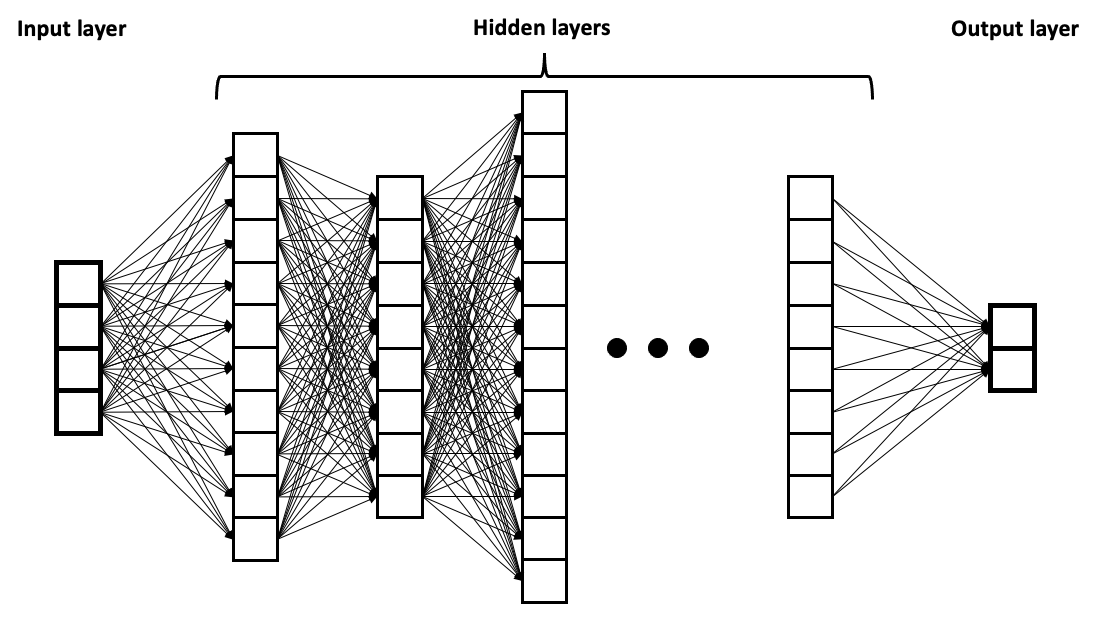
\includegraphics[width=0.75\linewidth]{deep_nn}
    \caption{Multilayer, fully-connected neural network. The squares in each layer correspond to the neurons, while the lines connecting them represent the weights $W^{(i)}_{a b}$. Each neuron implicitely has an associated nonlinear activation function, which somehow processes the input of the previous layer. \href{https://commons.wikimedia.org/wiki/File:Example_of_a_deep_neural_network.png}{Credit}}
    \label{fig:nn}
\end{figure}
Specifically, this is a representation of a \emph{fully-connected} neural network, i.e. one where each neuron of a given layer influences every neuron in the next layer, and vice-versa. The action of such a network can be expressed as a generalization of Eq. (\ref{eq:slnn_action}),
\begin{equation}
    f_W(X_{\mu})
    =
    \sigma^{(L)}\left(
        \sum_{a_L=1}^{p_L} W^{(L)}_{a_L a_{L-1}}
        \sigma^{(L-1)}\left(
            \sum_{a_{L-1}=1}^{p_{L-1}} W^{(L-1)}_{a_{L-1} a_{L-2}}
            \ \dots \ 
            \sigma^{(1)}\left(
            \sum_{a_{1}=1}^{p_{1}} W^{(1)}_{a_{1} \mu} X_{\mu a_{1}}
            \right)
        \right)
    \right),
    \label{eq:mlnn_action}
\end{equation}
where $L$ is the total number of layers and $p_i$, $\sigma^{(i)}$ and $W^{(i)}$ are the number of neurons, activation function and weight matrix of the $i$-th layer respectively. An element of the weight matrix $W^{(i)}_{a b}$ of the $i$-th layer gives the weight associated to the connection between the $a$-th neuron of this layer and the $b$-th neuron of the previous layer. The number of \emph{input features} of layer $i$ corresponds to the number of neurons in the previous layer.
Note that the first layer (called \emph{input layer}) "connects" to the data and hence has $d$ input features, while the last layer (called \emph{output layer}) corresponds to the output of the network.
One further defines, for a given sample $\mu$ and each layer $i$, the \textbf{pre-activations} and \textbf{post-activations} of its neurons:
\begin{align}
    h^{(i)}_{a_{i+1}\mu} &=
    \sum_{a_i=1}^{p_i} W^{(i)}_{a_{i+1}a_{i}} t^{(i-1)}_{a_{i}\mu} \\
    t^{(i-1)}_{a_{i}\mu} &=
    \sigma^{(i-1)}(h^{(i-1)}_{a_{i}\mu}) \\
    \text{with } t^{(0)}_{\mu} &= X_{\mu}.
\end{align}
Intuitively, $t^{(i-1)}_{a_{i}\mu}$ is what comes out of the $a_{i}$-th neuron of the previous layer and $h^{(i)}_{a_{i+1}\mu}$ is what comes into the $a_{i+1}$-th neuron of the current layer.

\subsubsection*{Activation Function and Losses}
Common examples of activation functions are
\begin{itemize}
    \item Rectified Linear Unit (ReLU), the most used choice:
    \begin{equation}
        \sigma(x) = \max(0,x)
    \end{equation}
    \item Hyperbolic Tangent
    \begin{equation}
        \sigma(x) = \tanh(x)
    \end{equation}
    \item Sigmoid Function
    \begin{equation}
        \sigma(x) = \frac{1}{1+e^{-x}}
    \end{equation}
    \item Threshhold Function: This is the one that most resembles a biological neuron
    \begin{equation}
        \sigma(x) = \Theta(x-\kappa).
    \end{equation}
\end{itemize}
The choice of a loss will depend a lot on the type of problem one is interested in. For regression, the most common loss is the well-known quadratic loss,
\begin{equation}
    l(y_{\mu}, f_W(X_{\mu}))
    =
    (y_{\mu} - f_W(X_{\mu}))^2.
\end{equation}
For classification into $K$ classes, the most common one is the cross-entropy loss,
\begin{equation}
    l(y_{\mu b}, f_W(X_{\mu}))
    =
    - \sum_{b=1}^{K}y_{\mu b} \ln{p_{\mu b}}
    \quad\quad
    p_{\mu b}
    =
    \text{softmax}\left(h^{(L)}_{b \mu}\right),
\end{equation}
with the softmax defined in Eq. (\ref{eq:softmax}). Note that in this context, the output layer $L$ naturally has $K$ neurons, corresponding to the $K$ categories. This is nothing but logistic regression, except that the input to the softmax is the activation of the output layer of the neural net.

\subsubsection*{Backpropagation}

\subsection{Convolutional Neural Networks}
\end{document}